\documentclass[a4paper,12pt]{article}
\usepackage[utf8x]{inputenc}

%opening
\title{Digital Logic Circuit simulator in python}
\author{Meghanad Shingate - 09307608,\\ Nirbhay Rane - 09307905,\\ Bharat Kumar - 09307904\\ Group - 13 \\ [10pt] AE 663 Course Project Report}

\usepackage{fancyhdr}
\usepackage{epsfig}
\usepackage{times}
\usepackage{bm}
\usepackage{amsmath,amssymb}
\usepackage{color}
\usepackage{array}
\usepackage{multirow}
\usepackage{subfigure}
\usepackage{listings}
\date{}


\lstset{ %
language=python,                  % the language of the code
basicstyle=\footnotesize\ttfamily,       % the size of the fonts that are used for the code
%numbers=left,                   % where to put the line-numbers
numberstyle=\footnotesize,      % the size of the fonts that are used for the line-numbers
stepnumber=1,                   % the step between two line-numbers. If it's 1, each line 
                                % will be numbered
numbersep=5pt,                  % how far the line-numbers are from the code
backgroundcolor=\color{white},  % choose the background color. You must add \usepackage{color}
showspaces=false,               % show spaces adding particular underscores
showstringspaces=false,         % underline spaces within strings
showtabs=false,                 % show tabs within strings adding particular underscores
frame=single,                   % adds a frame around the code
tabsize=2,                      % sets default tabsize to 2 spaces
captionpos=b,                   % sets the caption-position to bottom
breaklines=true,                % sets automatic line breaking
breakatwhitespace=false,        % sets if automatic breaks should only happen at whitespace
%title=\lstname,                 % show the filename of files included with \lstinputlisting;
                                % also try caption instead of title
escapeinside={\%*}{*)},         % if you want to add a comment within your code
morekeywords={*,...}            % if you want to add more keywords to the set
}

\begin{document}

\maketitle


\section{Introduction}

We have implemented  \textit{pydlcs},  a  Digital Logic Circuit simulator in python as a part of our course project. It is a nice simulation exercise to show power 
of object oriented programming in python. We have implemented following functionality in our simulator.

\begin{itemize}
 \item Basic gates - NOT, AND, OR, NAND.
\item Derived gates - XOR, XNOR.
\item Combinational Circuits - Half adder, Full adder, 1x2 MUX, 2x1 DEMUX.
\item Sequential Circuits - D, JK, T flip flops, latches, frequency divider, Shift register and counters.
\item Signal Sources -  clock, constant signal generator.
\end{itemize}

  
%%%%%%%%%%%% Chapter 2
\section{System Overview}

 

\begin{figure}[h]
   \begin{center}
   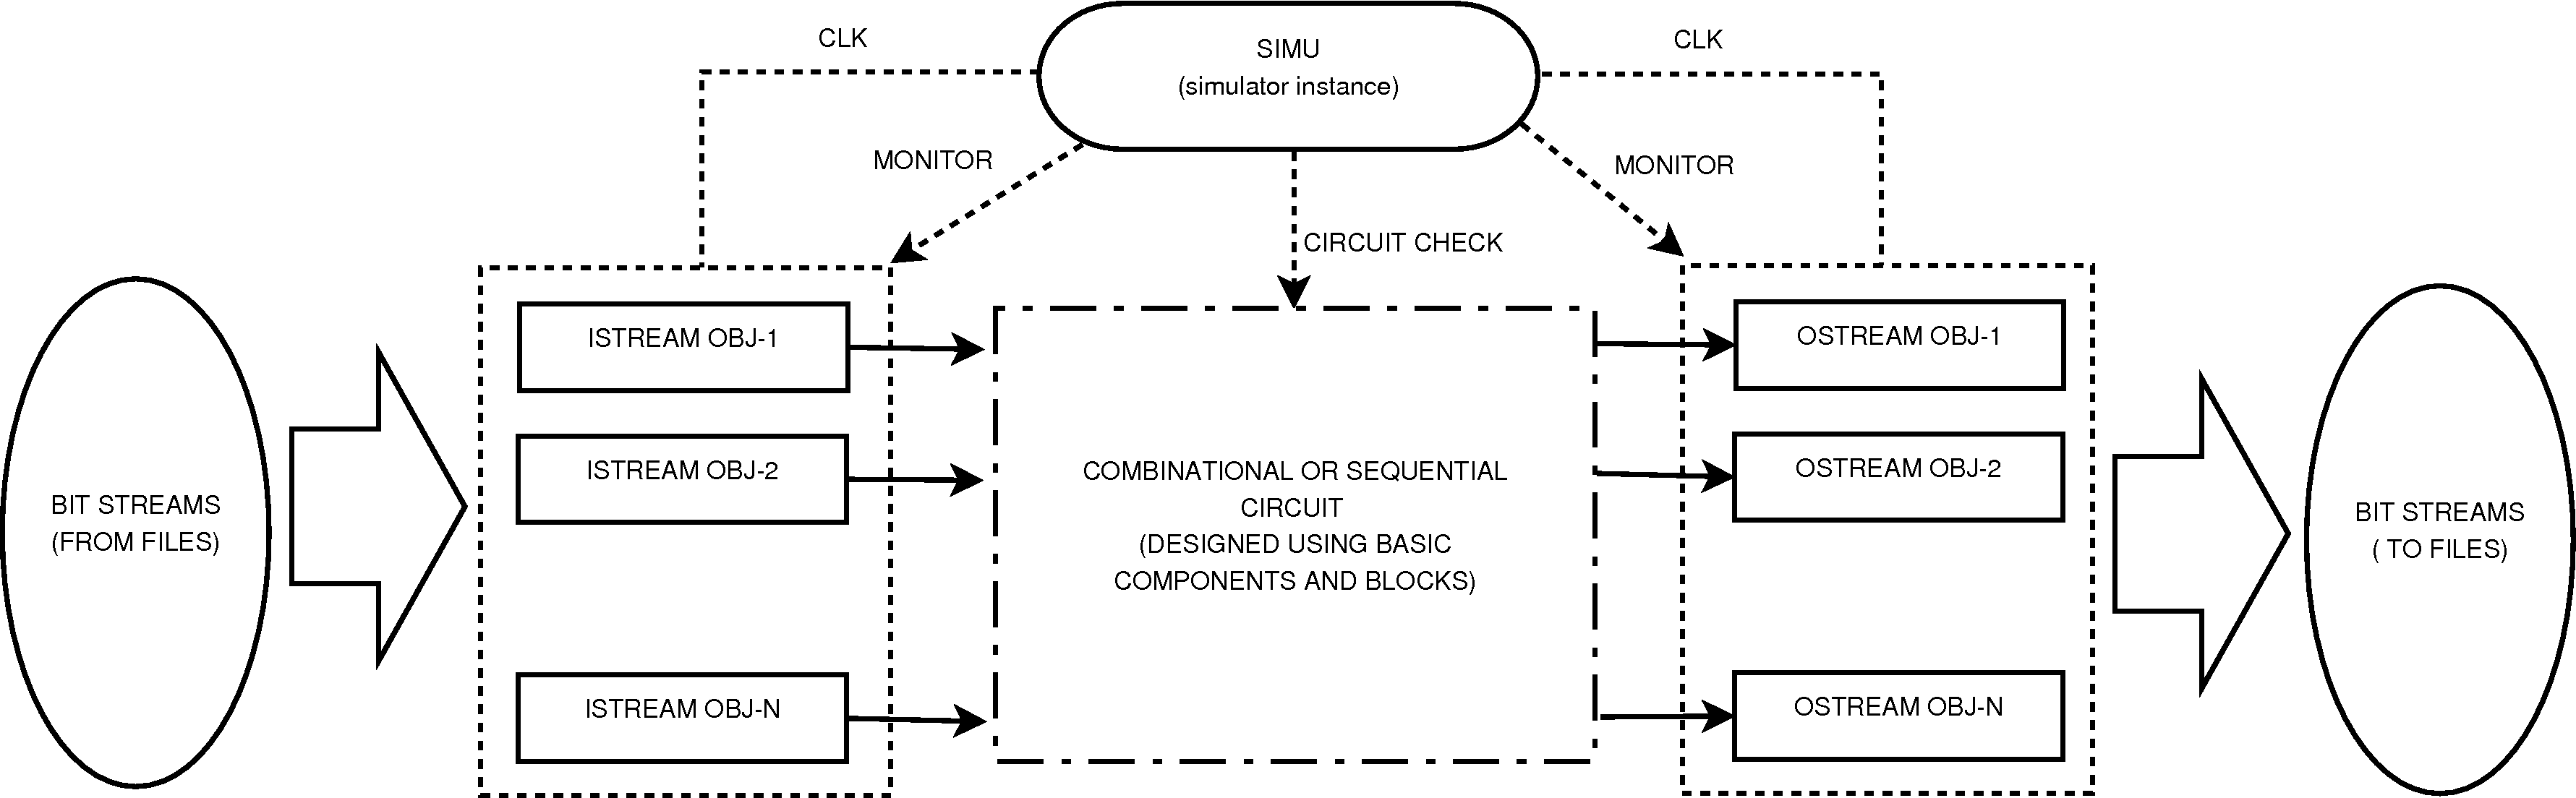
\includegraphics[scale=0.25]{syst_model.png}
    \caption{{Simulator System Model}}
  \label{syst_model}
  \end{center}
  \end{figure}





Figure \ref{syst_model} shows the system model of the \emph{pydlcs} simulator. Class \emph{SIMU} is the central class of the \emph{pydlcs} simulator. It monitors the whole circuit operations and provides clock to different elements of the circuit. Its main functions are,
\begin{itemize}
 \item Provide system clock to circuit elements
 \item Plotting input and output graphs
 \item Save the results and plots
 \item Monitor and control i/o streams
 \item Circuit debug option
\end{itemize}



 Simulator takes the bit-streams as an input form files specified. \emph{Istream} is the class defined for the providing the input facility from files. Each \emph{Istream} object is connected to one file on one side and can supply bit-stream to any number of gates of the circuit on other side. \emph{Ostream} is class defined for providing facility of writing result of simulation into the file specified. \emph{Ostream} class object is connected to circuit pin from one side and pins data is logged into the file specified on other side. Both classes, \emph{Istream} and \emph{Ostream}, need to provide system clock for their operation. Their are different flags in \emph{SIMU} class that we need to set for enabling different options \emph{e.g.} for enabling annotation  of plots we need to set flag \emph{pannotate} in \emph{SIMU} object. Flags details are as bellow,
\begin{itemize}
 \item \emph{plots} - Enable plots
 \item \emph{pannotate} - Enable plot annotation
 \item \emph{pclk} - Enable plotting system clock
 \item \emph{start} - Start the simulation flag
 \item \emph{stop} - Stop simulation flag
 \item \emph{debug} - Enable debugging
 \item \emph{step} - Enable step execution
\end{itemize}

 There should be only one instance of \emph{SIMU} class per circuit description file. Introduction to writing circuit description file is given in upcoming sections. 




\section{Implementation Details}

  \begin{figure}[h]
   \begin{center}
   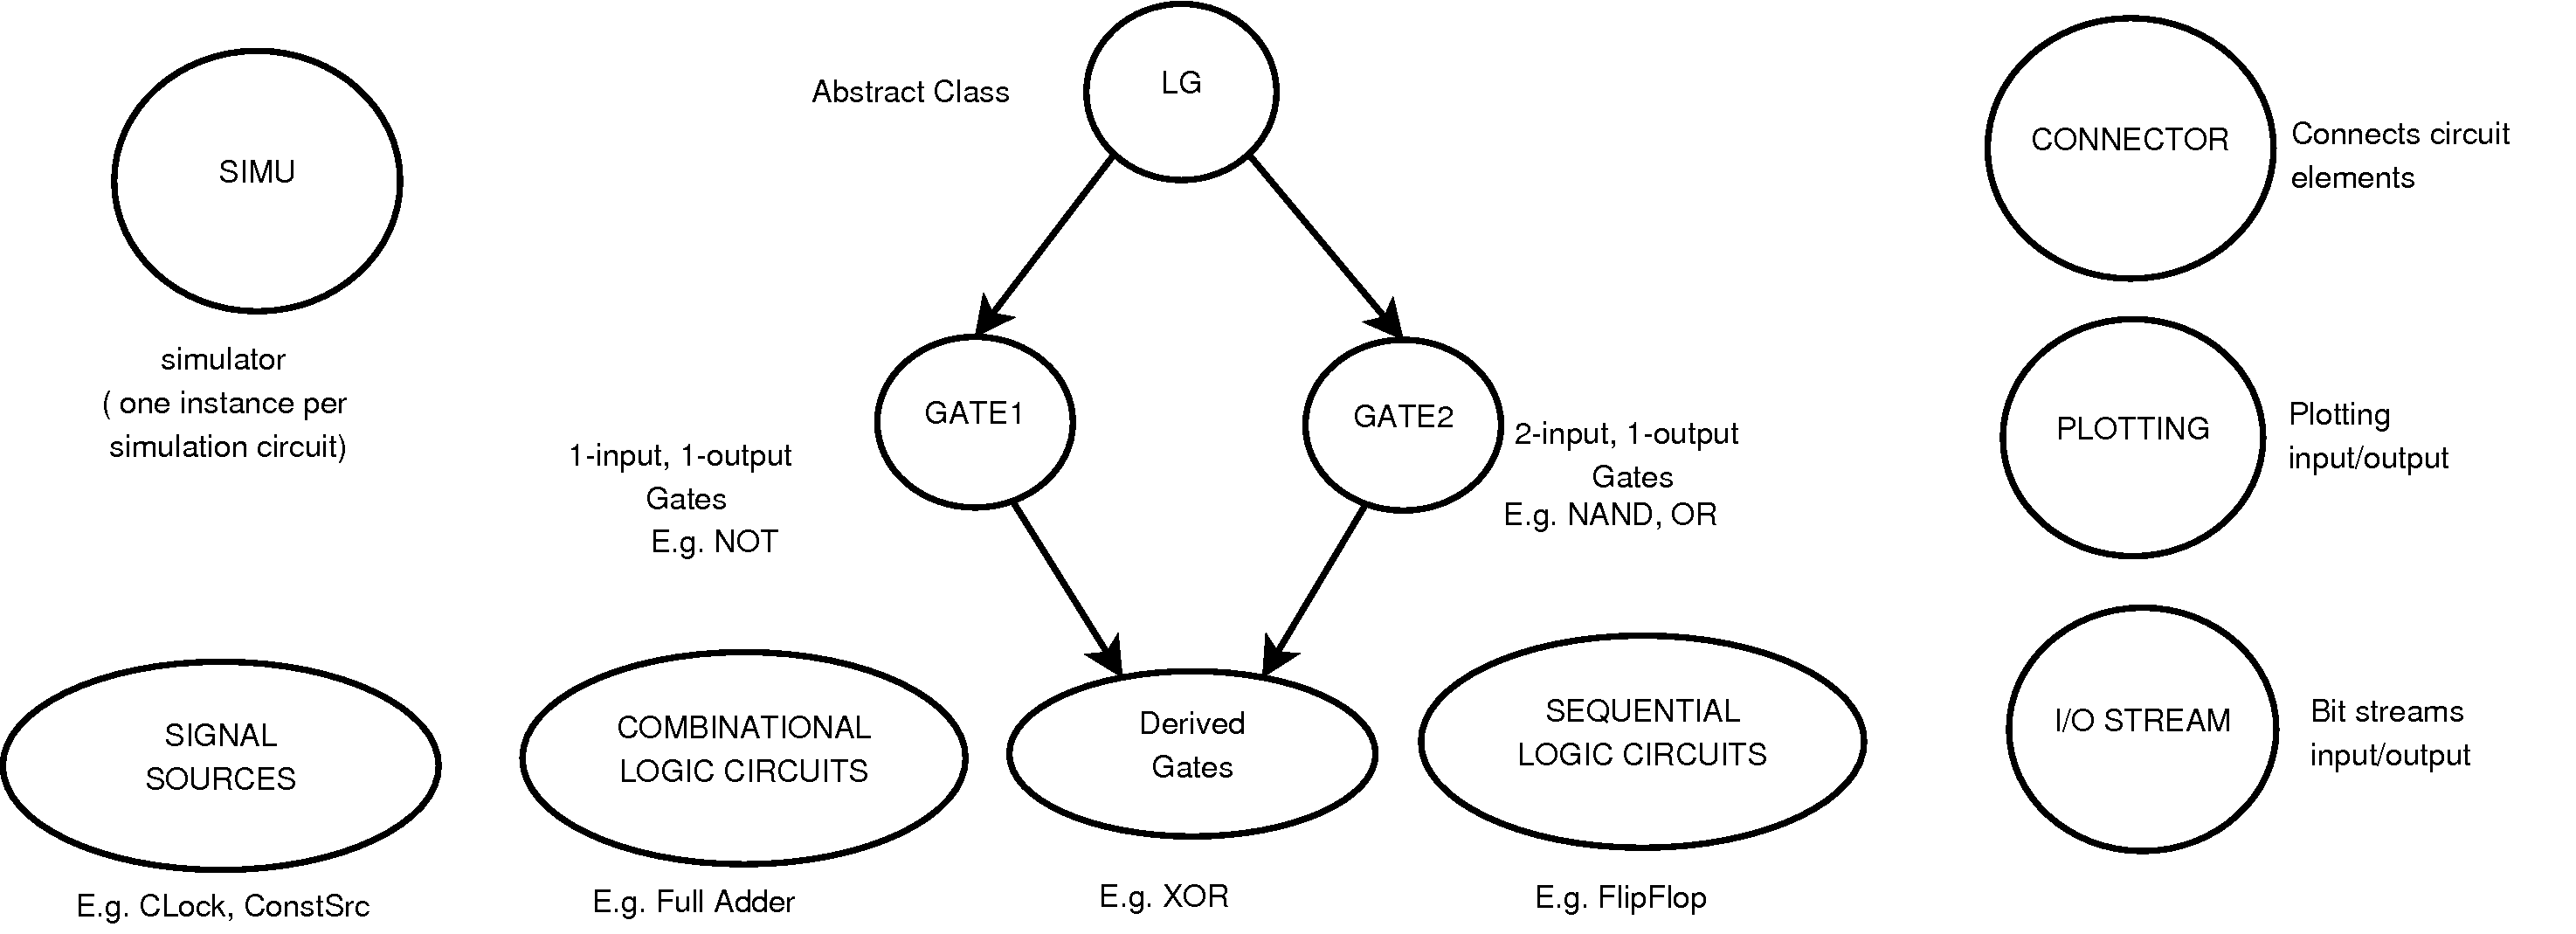
\includegraphics[scale=0.3]{class3.png}
    \caption{{Class Structure}}
  \label{class_struct}
  \end{center}
  \end{figure}

The implementation of Logic simulator is done using a modular and test driven approach. Each of the module is implement using a 
set of classes. The Logic simulator consists of the following classes.
\begin{itemize}
\item Class Logic Gate
\item Class Gate
\item Classes implementing basic gates.
\item Class Connector.
\item Classes implementing derived gates.
\item Classes implementing combinational logic circuits.
\item Classes implementing sequential elements.
\item Classes implementing signal sources and clocks.
\item Class I/O stream 
\item Class Simulator
\end{itemize}

\subsection{Class Logic Gate}
This is an abstract class which implements a method to name the gate that is created. 
This name is then used to refer to the pins of this gate and define the the pins to which it is connected. It also has the definition of an evaluate function. This function is overloaded by any class derived from this class. All the class which implement basic logic gates are derived from this class.\\

This code snippet shows its implementation.
\lstinputlisting[language=bash]{Logic_gate.py}

\subsection{Class Gate}
This class is derived from the abstract class Logic Gate. The purpose of this class is to create objects that represent the pins of a gate. In our implementation we have a class named GATE2 which creates terminals of a two input and one output logic gate. The input terminals are named A and B, Output terminal is named C.This implementation can be extended to create gate having arbitrary number of inputs and outputs.The Connector call creates a pin with a particular name and defines weather a change in this pin's value will activate the gate or not. Further details about Connector are provided subsection Connector.
The code below shows the implementation.
\lstinputlisting[language=bash]{Gate2.py}

\subsection{Classes implementing basic gates}
All the basic gates ie AND, OR, NAND etc are derived from the class GATE2 (except NOT which has a single input and output.). Each of these classes overloads the function evaluate defined in the class Logic Gate. The evaluate function is used to calculate the output of the gate by reading the corresponding inputs. \\

\subsubsection{NOT gate}

\begin{figure}[h]
\centering
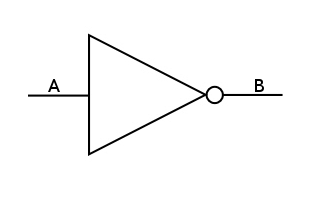
\includegraphics[scale=0.75]{NOT.png}%[width=8.5cm, height=7cm]{case1}
\caption{NOT gate}
\end{figure} 


\lstinputlisting[language=python]{not.py}

We can see that class NOT derived from LG class. It has two attributes for input and output pin. 
When a event happens on the input pin, evaluate method of this class is called which performs NOT operation.\\

The code below shows the implementation of AND gate.
\lstinputlisting[language=bash]{And.py}

Similarly we have implemented other basic gates like OR, NAND using above approach.

\subsection{Class Connector}
This class has no base class that is it is not a derived class. The pourpose of this class is to create pins , to name and initialize them and to attach them to a particular gate. Each of the pin has an attribute called owner which is used to denote the gate to which a pin is connected. The connector also takes arguments called activates and monitor. The activates is a attribute of the pin which tells if a change in the value of a pin activates the gate or not. By default activates is set to zero meaning that the pin will not activate the gate. The activation of the gate cause the function evaluate to execute which produces the output of the gate. The attribute monitor tell if we want to print the value of a pin or not. By default it is set to 0 which means it will not print the value of the pin. Apart from the initialization mentioned above the Connector class is also responsible to
\begin{itemize}
 \item connect the pins of one gate to another gate 
 \item print the value of a pin if its monotor attribute is set to 1 
\item set the value of the pins and to call the evaluate function of the appropriate object when it sees a change in the input pins of a particular gate.
\end{itemize}
The above three functions are implemented using the functions Set and Connect. Set is used to set the value of a pin and call the evaluate function of appropriate gate. This is done by simply calling the evaluate function of the owner of the pin. Connect is used to connect the pins of one gate to another , it dose this by storing all the pins which are connected to that pin in a list. whenever the value of a  particular pin changes set reads the connect list and it calls the evaluate function of all the gates corresponding to the pins stored in the connect list. \\

The code below shows the implementation of the connect function.

\lstinputlisting[language=bash]{Connector.py}

\subsection{Classes implementing derived gates}

We can see that class XOR is derived from class LG. It uses the basic gate objects of AND, NOT and OR to implement XOR functionality. XNOR gate can be 
easily implemented with little change in above logic. 


\begin{figure}[h]
\centering
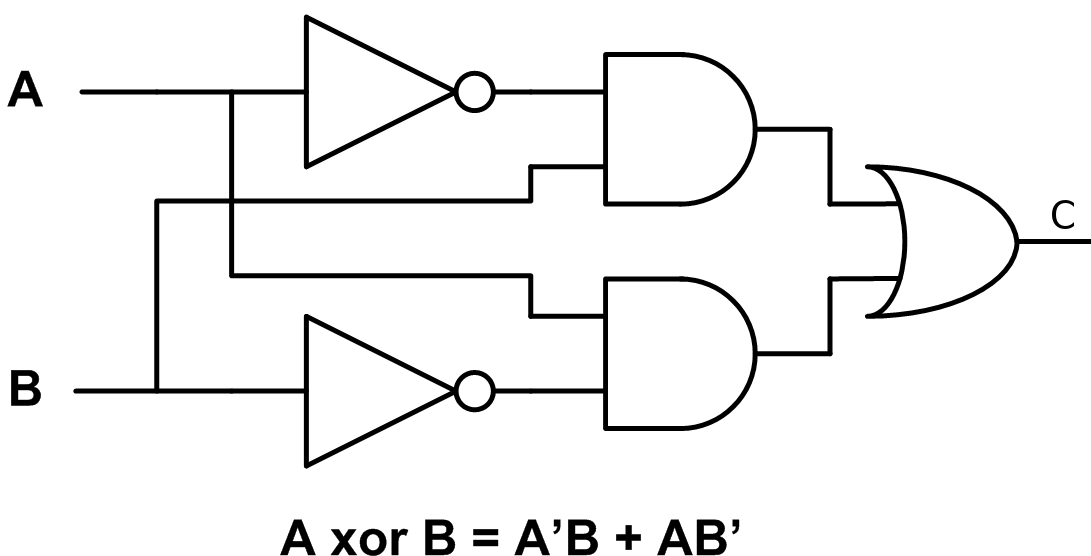
\includegraphics[scale=0.65]{XOR.png}%[width=8.5cm, height=7cm]{case1}
\caption{XOR gate}
\end{figure} 

\lstinputlisting[language=python]{XOR.py}


\subsection{Classes implementing combinational logic circuits}

In this section we describes the implementation of combinational logic circuits like half adder, full adder, MUX/DEMUX.

\subsubsection{Half Adder}

\begin{figure}[h]
\centering
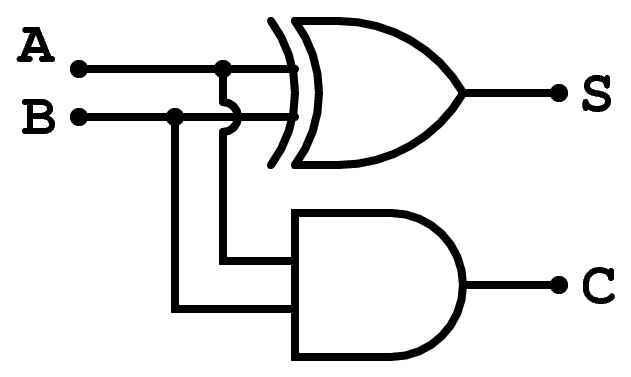
\includegraphics[scale=0.3]{halfadder.png}%[width=8.5cm, height=7cm]{case1}
\caption{Half Adder}
\end{figure} 

\lstinputlisting[language=python]{halfadder.py}

We can see that class HalfAdder is derived from class LG. It uses the gate objects of XOR, AND to implement half adder functionality.

\subsubsection{Full Adder}

Similarly we have implemented Full Adder class using HalfAdder class objects and OR gate object.

\begin{figure}[h]
\centering
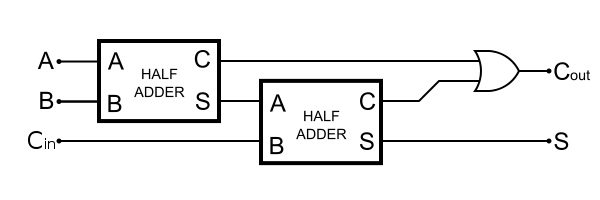
\includegraphics[scale=0.5]{fulladder.png}%[width=8.5cm, height=7cm]{case1}
\caption{Full Adder}
\end{figure} 

\lstinputlisting[language=python]{fulladder.py}


In addition we have implemented 2x1 MUX and 1x2 DEMUX classes using the basic gate objects.

\subsection{Classes implementing sequential logic elements}

In this section we describes the implementation of sequential logic circuits like Flip-Flops, counters.

\subsubsection{JK Flip Flop}

As an example we show implementation of JK Flip Flop class which is derived from LG class.

\begin{figure}[h]
\centering
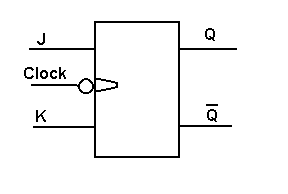
\includegraphics[scale=0.75]{jkflop.png}%[width=8.5cm, height=7cm]{case1}
\caption{Full Adder}
\end{figure} 

\lstinputlisting[language=python]{jk.py}

It has four attributes for J, K input pins, clcok input and Q output. When a event happens on clock pin, evaluate method of this class is called 
which performs JK flip flop operation.

Similarly we have implemented D and T Flip Flops. Also counter and shift register circuits are designed using this flip flop objects.


\subsection{Class I/O stream }


\begin{figure}[h]
   \begin{center}
   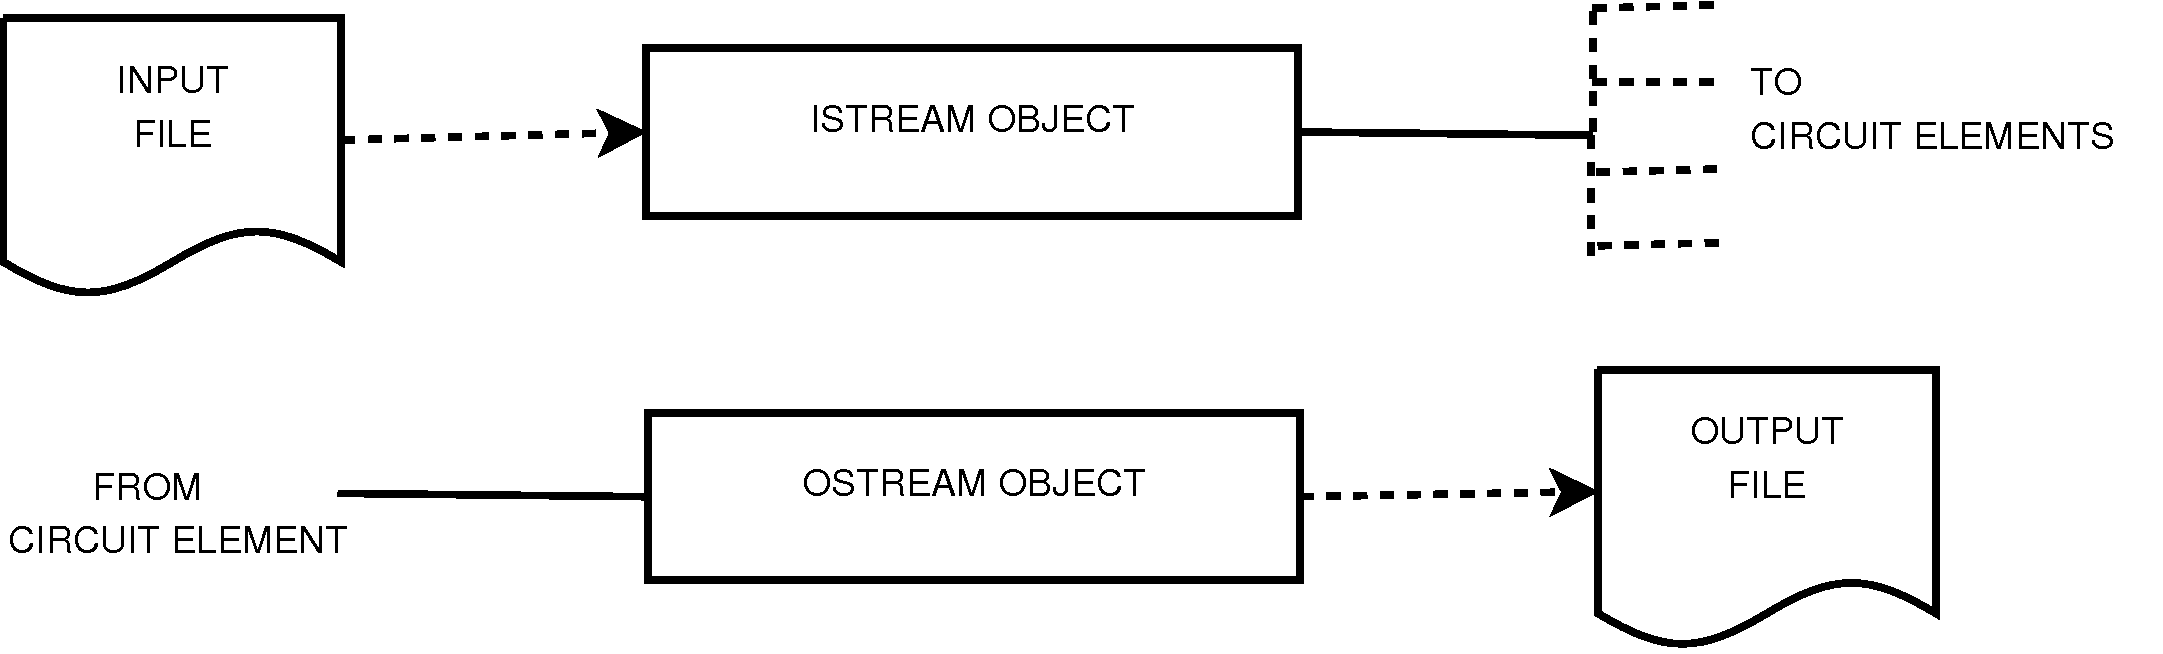
\includegraphics[scale=0.3]{iostream.png}
    \caption{{I/O Stream Model}}
  \label{iostream}
  \end{center}
  \end{figure}
 

\subsection{Class Simulator}
We have implemented the simulator in class SIMU. The following diagram shows the functional overview of the simulator. Figure \ref{class_struct}  shows the overall class structure of the simulator design. 

\begin{figure}[h]
   \begin{center}
   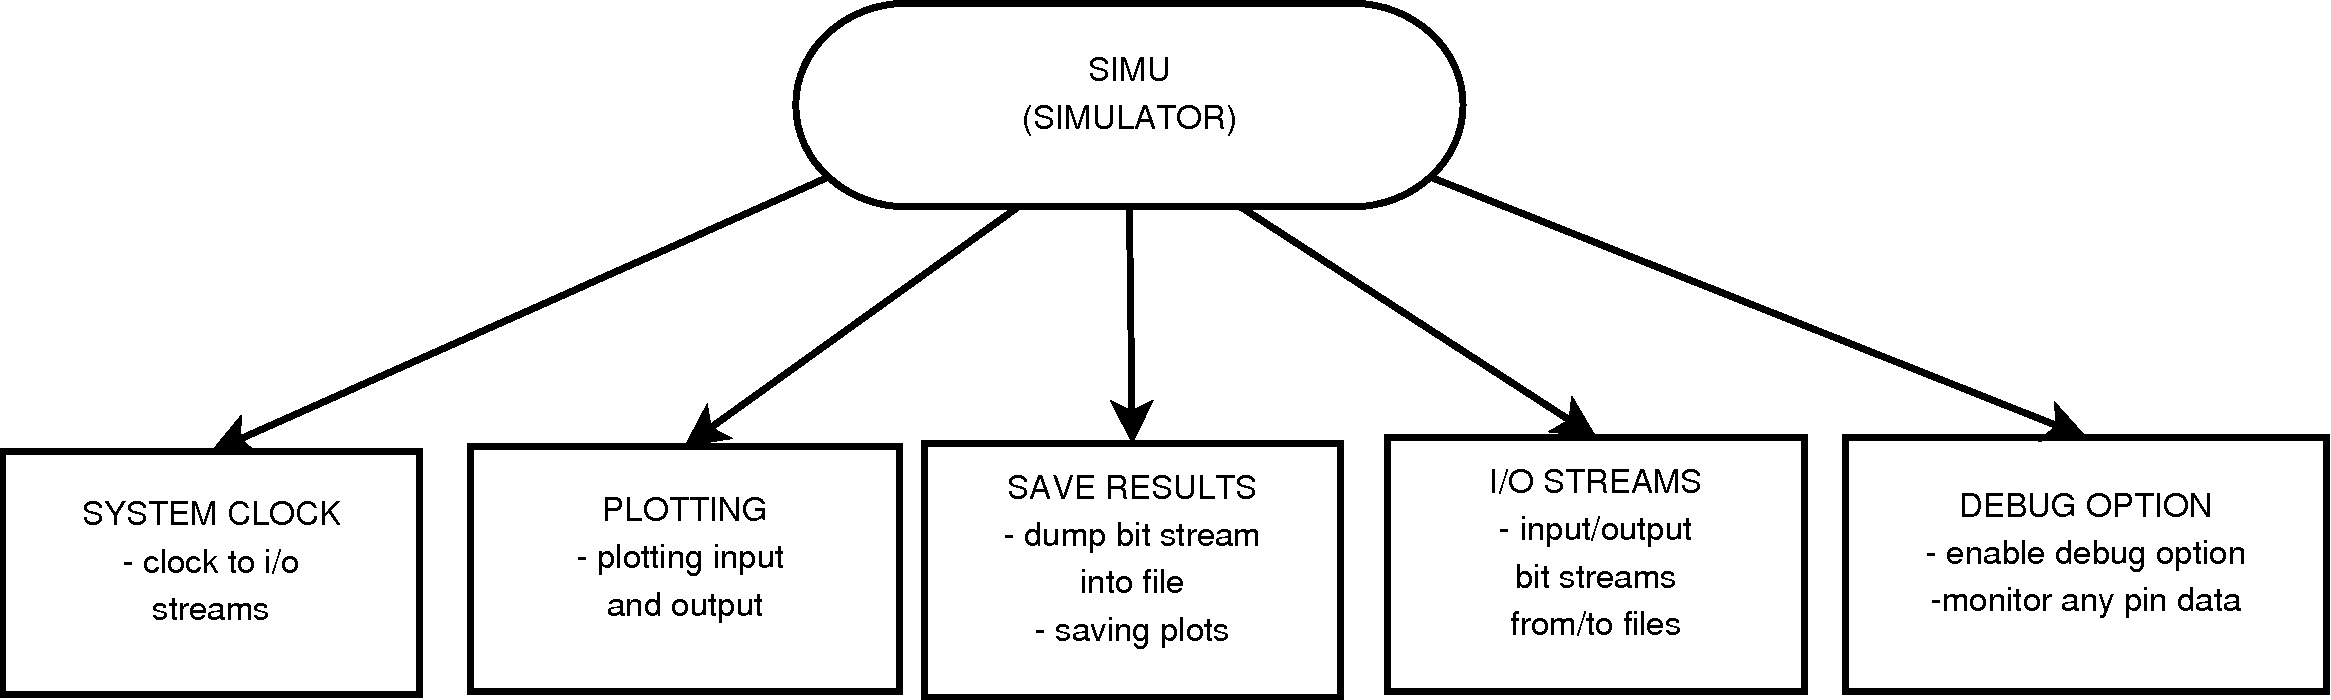
\includegraphics[scale=0.35]{simu_model.png}
    \caption{{Simulator Class Details}}
  \label{simu_class}
  \end{center}
  \end{figure}


\subsection{Clocks \& signal sources classes}
The clocks and sources are nothing but classes which create instances of the Ostream class and perform required operations to generate the output. The output is generally a sequence of alternating ones and zeros or data read from a file.
 


\section{Writing a circuit description for given logic circuit}

In this section we present the our method of writing scripts to simulate given logic circuit using above mentioned modules like basic gate, combinational and 
sequential circuit modules. We will take a following example of 4 bit synchronous binary counter for this purpose.  

\begin{figure}[h]
\centering
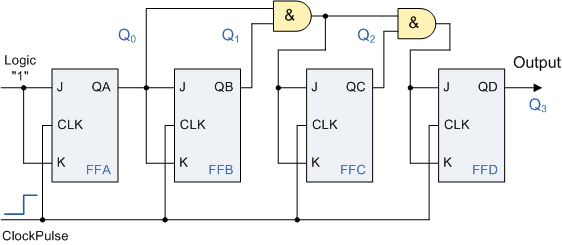
\includegraphics[scale=0.6]{cou4.png}%[width=8.5cm, height=7cm]{case1}
\caption{Binary 4-bit Synchronous Counter}
\end{figure}

To simulate this logic circuit we need 4 JK Flip Flops, 2 AND gates, constant source (CO) of generating input 1, clock source and 4 output streams.
We generate above required objects different classes described in previous sections. Here we have to connect clock such that all flip flops are clocked 
simultaneously. We do that by output of clock (sim.clk.out) to each flip flops clock. We have to maintain the right order in connecting the clock. Using connector class objects 
we have connected each component of circuit as shown in figure. Finally we start the simulation using object sim of SIMU class. 

\lstinputlisting[language=python]{expl_4bit_Sync_Binary_counter.py}

The counter output is shown in the Fig. \ref{op}.
\begin{figure}[t]
\centering
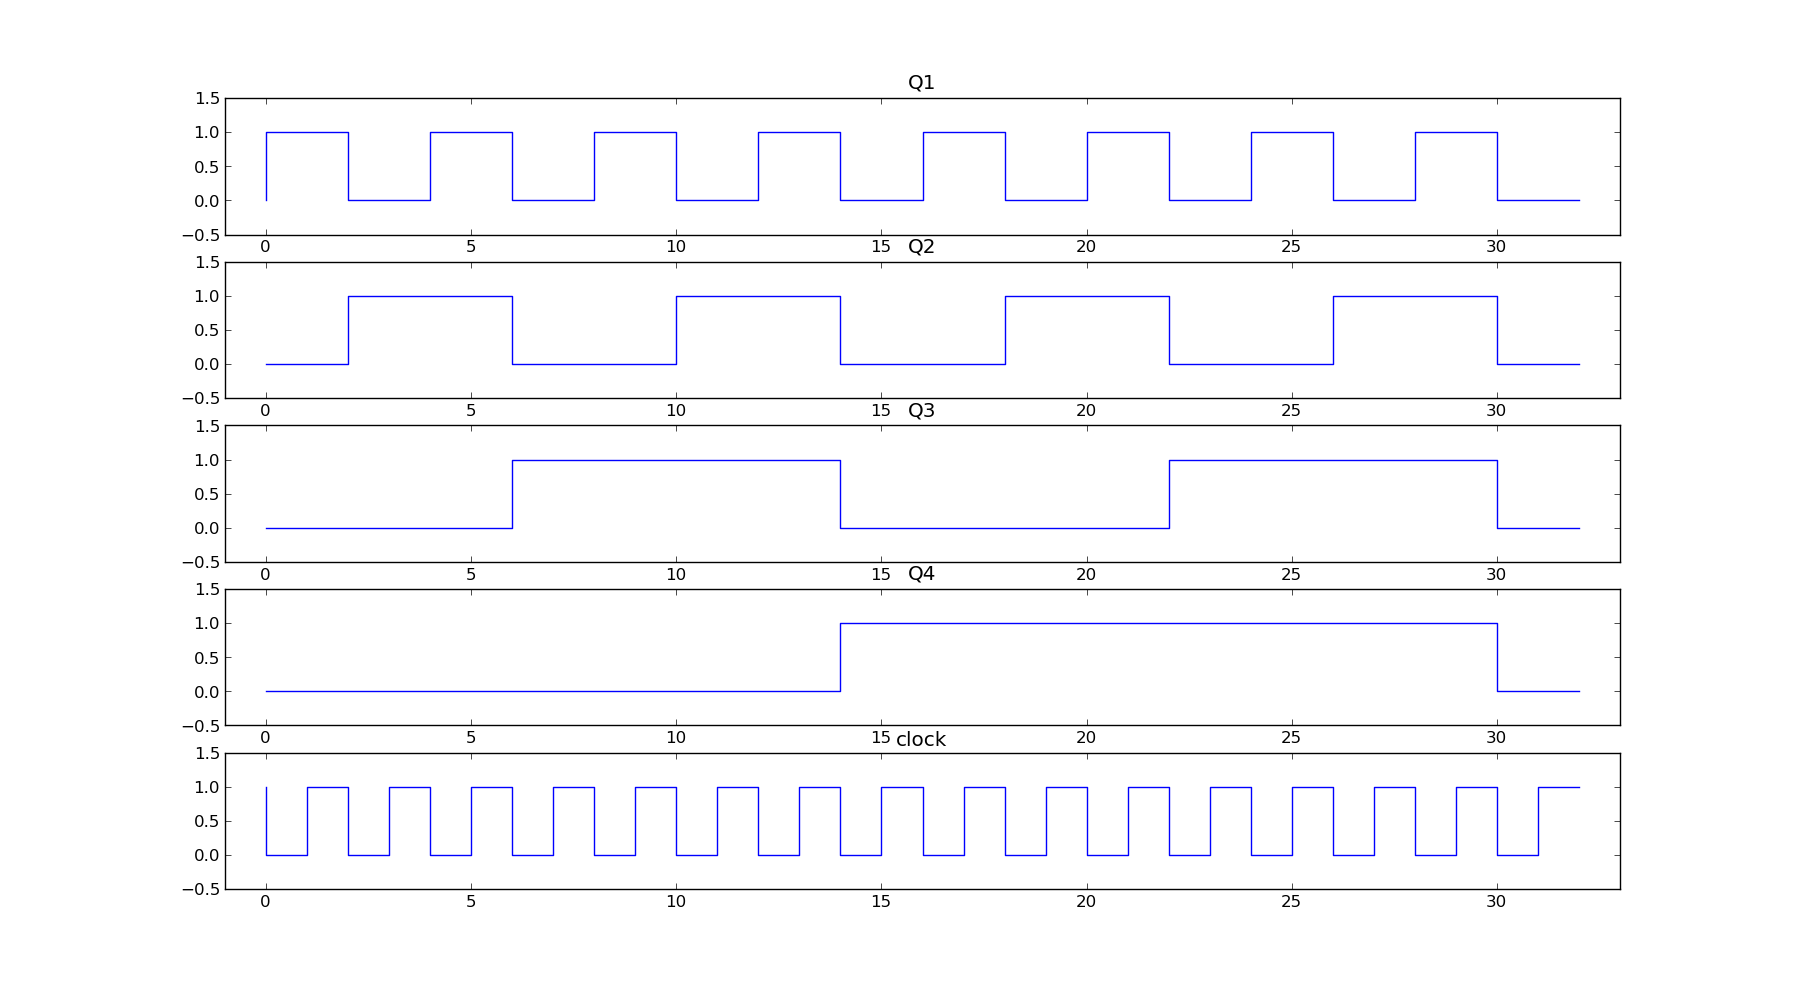
\includegraphics[scale=0.35]{counter_op.png}%[width=8.5cm, height=7cm]{case1}
\caption{Binary 4-bit Synchronous Counter Output}
\label{op}
\end{figure}

\pagebreak
 \section{Conclusion \& future work}
We have successfully implemented a digital logic simulator in python. We have demonstrated simulation of logic circuit containing combinational and sequential elements using our simulator. Potential future work includes GUI implementation. Feedback that activates the evaluation function is not possible in current release, this can be done as future work.


\end{document}
